% slides.tex: full-length (~75 min) version of the talk.
% https://pascalmichaillat.org/d1/
%
% Every number quoted here is a macro from output/results/slide-numbers.tex,
% which is generated by program/write-slide-macros.R off the same results
% layer that paper.Rmd reads.  Do not hard-code an estimate: add it to the
% generator.  `make slides.pdf` refreshes the macros first.

\documentclass[11pt,xcolor={dvipsnames},hyperref={pdftex,pdfpagemode=UseNone,hidelinks,pdfdisplaydoctitle=true},usepdftitle=false,aspectratio=169]{beamer}
\usepackage{tikz}
\usetikzlibrary{positioning}

\usepackage{presentation}

\input{output/results/slide-numbers}

\newcommand{\gc}[1]{{\footnotesize\textcolor{gray}{#1}}}

\usepackage{natbib}
\usepackage{verbatim}
\usepackage{threeparttable}

\hypersetup{pdftitle={The Returns to Climate Adaptation in Manufactured Housing}}
\newcommand{\pdf}{paper}

\begin{document}

\title{The Returns to Climate Adaptation in Manufactured Housing}
\information%
{Colin Williams}%
{University of Virginia -- \today}

\begin{frame}
\titlepage
\end{frame}

%% ============================================================
%% MOTIVATION
%% ============================================================

\begin{frame}[plain]
    \centering
    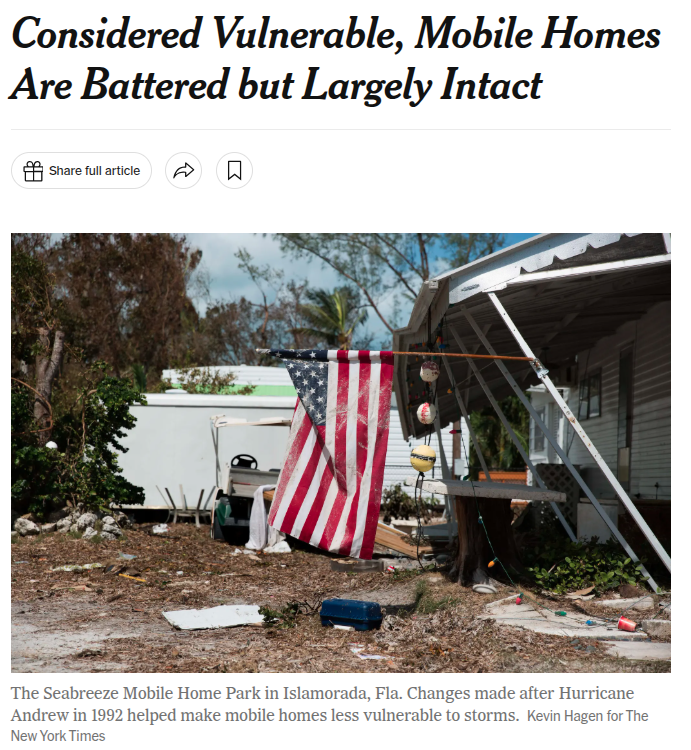
\includegraphics[width=\paperwidth,height=\paperheight,keepaspectratio]{motivation/nyt_irma_20170914.png}
\end{frame}

\begin{frame}[plain]
    \centering
    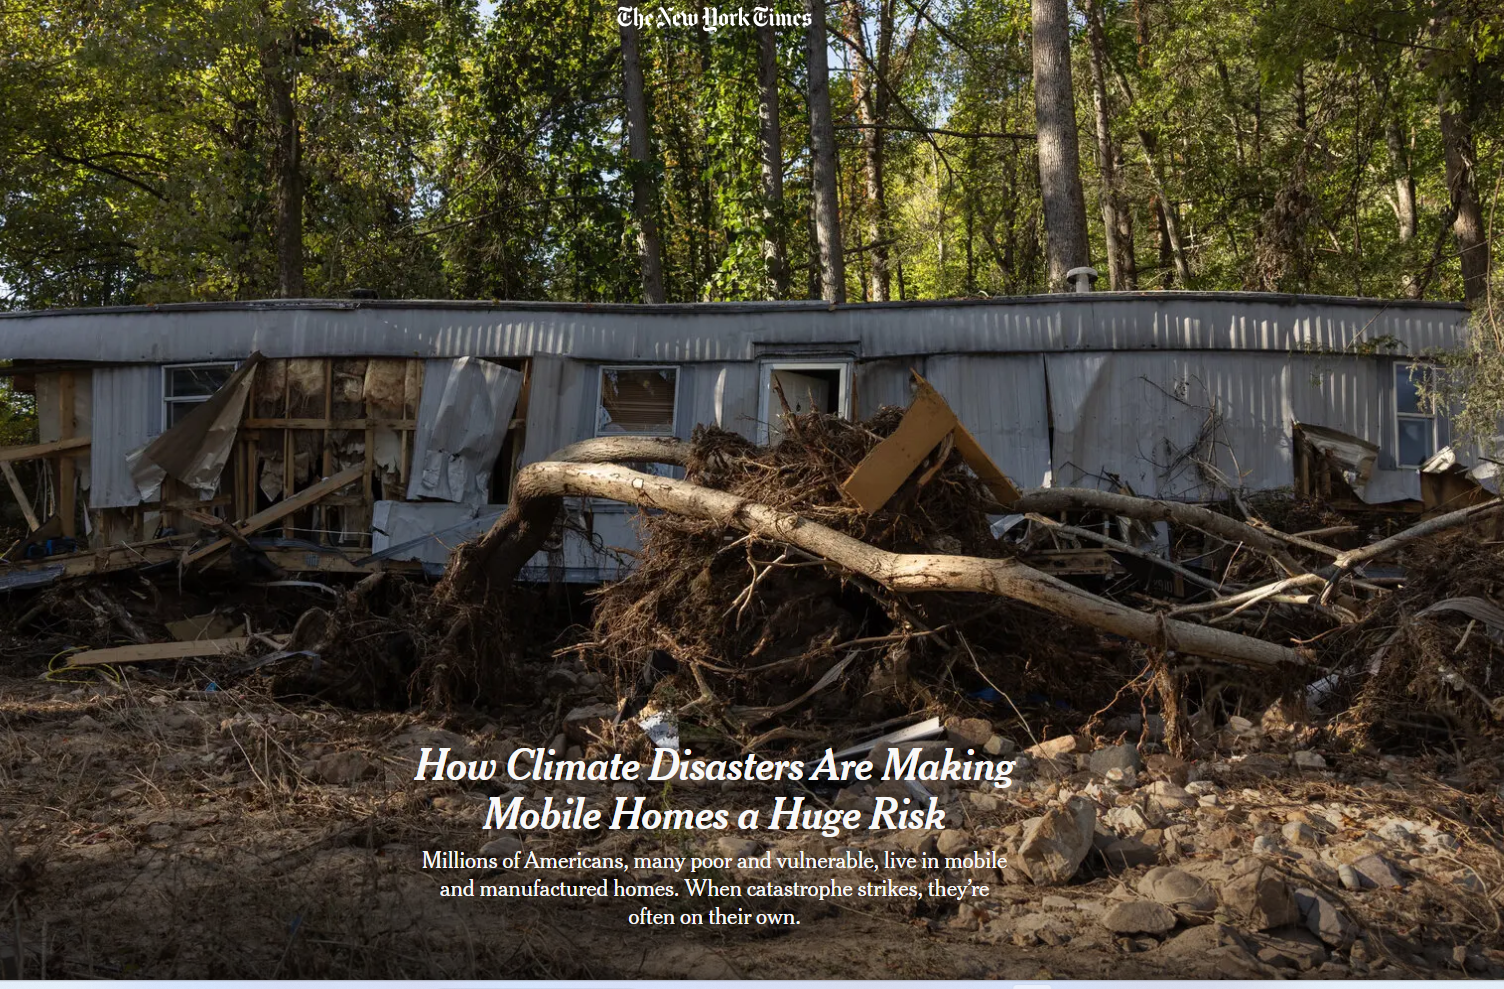
\includegraphics[width=\paperwidth,height=\paperheight,keepaspectratio]{motivation/nyt_mh_hurricanes_20241014.png}
\end{frame}

\begin{frame}[t]
    \frametitle{(How) are mobile homes at risk from climate change?}

    \vspace{0.8em}

    Three sources of risk:

    \begin{enumerate}
        \item Physical characteristics: elevation, anchoring, fastening, etc.
        \item Location (location, location...)
        \item Policy: some disaster relief targeted at \al{landowner}, not resident
    \end{enumerate}

    \vspace{0.6em}
    \pause

    This paper evaluates \#1: How does HUD code affect the cost and resilience of mobile homes?

\end{frame}

\begin{frame}
    \frametitle{Why now?}

    \textbf{The ROAD to Housing Act (2025)} removes the \al{permanent steel chassis} requirement

    \begin{itemize}
        \item Few manufactured homes (MH) moved after installation
        \item Chassis adds \$5-10k cost for little benefit
    \end{itemize}

    \vspace{1em}
    \pause

    \textbf{MH wind standards, dating to 1994, assume a chassis}
    \begin{itemize}
        \item anchoring and stabilization tie to the steel frame; piers bear on the main rails \gc{(24 CFR \S 3280.306; installation standards at Part 3285)}
        \item HUD is about to rewrite the wind standards
    \end{itemize}

    \vspace{1em}
    \pause

    \begin{large}
    How effective are current HUD wind standards?
    \end{large}

    % TODO: verify the enacted text and section numbering before circulating.
\end{frame}

\begin{comment}
\begin{frame}[t]
    \frametitle{When does a quality mandate raise welfare?}

    Any justification has to \al{name a specific failure}:

    \vspace{0.6em}

    \begin{itemize}\setlength{\itemsep}{0.35em}
        \item \al{Externalities.} Wind-borne debris damages neighbors \gc{\citep{baylis_mandated_2021}}
        \item \al{Fiscal externality.} Losses are partly socialized \emph{ex post} --- FEMA IA, SBA, subsidized NFIP \gc{\citep{deryugina_fiscal_2017, solomon_optimal_2026}}
        \item \al{Unobservable quality.} Buyers cannot inspect strap schedules or fastener spacing
        \item \al{Missing insurance market.} Premiums do not price mitigation \gc{\citep{wagner_adaptation_2022}}
        \item \al{Misperceived risk / internalities.} \gc{\citep{bakkensen_going_2022, gallagher_learning_2014}}
        \item \al{Credit constraints.} Positive-NPV investment the buyer cannot finance
    \end{itemize}

\end{frame}
\end{comment}

\begin{frame}
    \frametitle{This paper}

    \begin{enumerate}\setlength{\itemsep}{1.0em}
        \item \begin{large}\textbf{Cost.} The 1994 wind standard raised MH prices by \al{\$\vPriceEff} (\vPriceEffPct\%) in treated states

        \item \begin{large}\textbf{Benefit.} Post-1994 MH sustain \al{\vBldgDmgPct\%} less building damage per flood claim \gc{(s.e.\ \vBldgDmgSELP\ log points)}\end{large}
        \begin{itemize}
            \item \$\vBldgDmgDol\ against a \$\vBldgDmgBase\ pre-1994 MH mean
            \item measured on flood losses (not wind) \so\ resilience spills across hazards
        \end{itemize}

        \item \begin{large}\textbf{Margin.} The reform changed \al{severity}, not \al{frequency}\end{large}
        \begin{itemize}
            \item damage per claim falls; claims per policy-year and take-up do not move
            \item and post-1994 MH policies sit \emph{more} often in floodplains
        \end{itemize}
    \end{enumerate}

    \vspace{1.0em}

    \so\ Flood alone returns \al{\vBCRPct\%} of the price increase. The reform targeted wind.

\end{frame}

\begin{frame}
    \frametitle{Literature}

    \footnotesize

    \textbf{Returns to building codes for disaster resilience}
    \begin{itemize}
        \item Florida hurricane codes, conflicting results \gc{\citep{simmons_economic_2018, dehring_coastal_2013}}
        \item descriptive work on the 1994 HUD reform \gc{\citep{simmons_manufactured_2008, kevin_r_grosskopf_manufactured_2005}}
        \item wildfire codes in California \gc{\citep{baylis_mandated_2021}}
    \end{itemize}

    \hspace{1em} \so \textbf{New:} MH are regulated \al{federally}, so code exposure separates from vintage

    \vspace{0.7em}

    \textbf{Identifying code effects}
    \begin{itemize}
        \item designs relying on across-vintage or across-location comparisons \gc{\citep{jacobsen_are_2013, levinson_how_2016}}
    \end{itemize}

    \hspace{1em} \so \textbf{New:} a \al{double difference in vintage $\times$ housing type} --- same county, same flood, same construction year

    \vspace{0.7em}

    \textbf{Adaptation, insurance, and the fiscal cost of disasters}
    \begin{itemize}
        \item risk misperception \gc{\citep{bakkensen_going_2022, gallagher_learning_2014}}; premiums and mitigation \gc{\citep{wagner_adaptation_2022}}
        \item fiscal spillovers of disasters and relief \gc{\citep{deryugina_fiscal_2017, baylis_moral_2019, solomon_optimal_2026}}
    \end{itemize}

    \hspace{1em} \so \textbf{New:} a mandated-adaptation \al{cost and benefit measured on the same reform}

\end{frame}

\begin{frame}
    % disclaimer -- get ahead of the "so was it worth it?" question
    \frametitle{Missing: most of the benefits}

    \begin{large}This paper does \al{not} evaluate the 1994 reform.\end{large}

    \vspace{1.2em}

    I measure \al{one} benefit channel, and it is not the targeted one:

    \begin{itemize}\setlength{\itemsep}{0.4em}
        \item \textbf{wind damage} --- what the standard was written for \gc{(not measured)}
        \item \textbf{uninsured losses} --- most MH carry no flood policy \gc{(not measured)}
        \item \textbf{displacement, lost income, injury} \gc{(not measured)}
        \item \textbf{insurance value} to risk-averse, credit-constrained households \gc{(not measured)}
        \item \textbf{\emph{ex post} relief spillovers} --- FEMA IA, SBA \gc{(not measured)}
    \end{itemize}

    \vspace{1.2em}

    \so\ What I deliver: a credible \al{cost}, a credible \al{lower bound} on benefits in an untargeted hazard, and evidence that structural standards have \al{cross-hazard} spillovers.

\end{frame}

%% ============================================================
%% INSTITUTIONS & DATA
%% ============================================================

\begin{frame}
    \heading{Institutions \& Data}
\end{frame}

\begin{frame}
    \frametitle{Manufactured housing and the HUD Code}

    \textbf{$\sim$6\% of the housing stock}; over 15\% in parts of the rural Southeast
    \begin{itemize}
        \item 22 million residents, disproportionately low-income and underinsured
        \item Hurricane Andrew (1992) destroyed \al{97\%} of MH in its path in Dade County, vs.\ 11\% of site-built \gc{\citep{noauthor_florida_1995}}
    \end{itemize}

    \vspace{0.8em}
    \pause

    \textbf{The 1994 reform.} HUD revised the Manufactured Home Construction and Safety Standards:
    \begin{itemize}
        \item three \al{wind zones}; structural upgrades required in Zones II and III
        \item stronger anchoring and strapping, upgraded sheathing and fastening, component and cladding wind-pressure requirements
        \item effective \al{July 1994}
    \end{itemize}

    \vspace{0.8em}
    \pause

    \textbf{The institutional feature that makes this work:} the HUD Code is a \al{federal} standard that \al{preempts} state and local regulation.

    \gc{Site-built homes in the same county remain under state and local codes \so\ a clean comparison group.}

\end{frame}

\begin{frame}
    \frametitle{Treated states: any \al{Zone II or III} county}
    \centering
    \includegraphics[width=\linewidth,height=0.80\textheight,keepaspectratio]{output/descriptives/map-mhs-treated-states.pdf}

    \vspace{-0.3em}

    \footnotesize{Control states are Zone I. Treatment is coarse: only about a third of the treated states' MH stock actually sits in a Zone II/III county.} \hfill \hyperlink{frame:windzone-intensity}{\beamerbutton{intensity}}
\end{frame}

\begin{frame}
    \frametitle{Flood insurance and manufactured homes}

    \textbf{The NFIP} insures flood risk in participating communities; purchase is \al{mandatory} for federally backed mortgages in Special Flood Hazard Areas.

    \vspace{0.8em}
    \pause

    \textbf{But MH mostly fall outside that mandate.}
    \begin{itemize}
        \item frequently financed with \al{chattel loans} --- secured by the home, not the land --- much of which is not federally related lending
        \item take-up: \al{\vPolMhPre} policies per 1,000 MH per year vs.\ \al{\vPolSbPre} per 1,000 site-built
    \end{itemize}

    \vspace{0.8em}
    \pause

    \textbf{Consequence for this paper.} MH are \al{\vMhClaimSharePct\%} of claims (\vNMhClaims\ of \vNAllClaims) and \vMhPolicySharePct\% of policies, against $\sim$6\% of the stock.

    \vspace{0.4em}

    \gc{Everything I estimate is measured on the \emph{insured} minority --- more selected and more financially connected than the population the motivation highlights. I return to this.}

\end{frame}

\begin{frame}
    \frametitle{Data}

    \textbf{Cost side: Census \al{Manufactured Housing Survey}}, state $\times$ year, 1988--2000
    \begin{itemize}
        \item average sales price by home size (single- vs.\ multi-section) and placement counts
        \item treated = states containing HUD wind Zone II or III; control = Zone I
        \item \al{\vNIndex} of \vNRaw\ state-years where both size-specific prices are published
    \end{itemize}

    \vspace{0.7em}
    \pause

    \textbf{Benefit side: FEMA \al{OpenFEMA} NFIP claims and policies}
    \begin{itemize}
        \item claims: loss date, construction year, building and contents damage, payments, tract
        \item policies: coverage, premium, flood zone, elevation \gc{(records begin 2009)}
        \item both flag manufactured homes
    \end{itemize}

    \vspace{0.7em}
    \pause

    \textbf{Sample.} Construction years \al{1984--1999}, losses from 1994; detached single-family residential only; continental US; deflated to \al{2000 dollars}.
    \begin{itemize}
        \item construction years binned in 2s, loss years in 5s \gc{(MH claims are rare)}
        \item reference bin: \al{1992--1993}
    \end{itemize}

\end{frame}

\begin{frame}\label{frame:sumstats}
    \frametitle{Summary statistics: NFIP}

    \footnotesize{
        \begin{table}
        \centering
        \input{output/descriptives/sumstats-nfip.tex}
        \end{table}
    }

    \vspace{0.3em}

    \tiny{Note: Policy panel 2009--2023; claims 1994--2023. Both restricted to construction years 1984--1999 and single-family residential. Shares and claim rate are policy-weighted. Damage in thousands of 2000 dollars.}
\end{frame}

%% ============================================================
%% EMPIRICAL STRATEGY
%% ============================================================

\begin{frame}
    \heading{Empirical Strategy}
\end{frame}

\begin{frame}
    \frametitle{Cost: a difference-in-differences across \al{wind zones}}

    $$P_{st} = \alpha_s + \gamma_t + \sum_{k \neq 1993} \beta_k \left(\mathbf{1}[\text{year} = k] \times \al{\text{Treated}_s}\right) + \varepsilon_{st}$$

    \vspace{0.5em}

    \begin{itemize}\setlength{\itemsep}{0.35em}
        \item $P_{st}$: fixed-weight MH price index in state $s$, year $t$ \gc{(next slide)}
        \item $\text{Treated}_s$: state contains a Zone II or III county
        \item 1993 omitted; $\alpha_s$, $\gamma_t$ state and year fixed effects
        \item weighted by mean 1988--1993 placements; SEs clustered by state
    \end{itemize}

    \vspace{1em}
    \pause

    The same specification, same sample, and same weights are used for \al{log placements}, so the price and quantity effects describe \al{one panel} rather than two.

\end{frame}

\begin{frame}
    \frametitle{Why a \al{fixed-weight} price index}

    The survey publishes an average price for single-section homes, for multi-section homes, and \al{across all homes placed}.

    \vspace{0.5em}

    \gc{Multi-section homes cost \$\vAvgPriceDouble\ against \$\vAvgPriceSingle\ for single-section --- a ratio of \vPriceRatio\ to 1.}

    \vspace{0.8em}
    \pause

    \so\ The all-homes average rises when \al{prices} rise \emph{or} when the \al{mix} shifts toward multi-section. A mix shift would enter the DiD as a price effect.

    \vspace{1em}

    $$P_{st} = \omega^{S} p^{S}_{st} + \omega^{D} p^{D}_{st}, \qquad \omega^{S} = \vWtSingle,\ \ \omega^{D} = \vWtDouble$$

    \vspace{0.5em}
    \pause

    Weights are \al{national 1988--1993 shares}, held fixed across all states and years.

    \begin{itemize}
        \item the index is the cost of a \al{fixed basket}: no variation in the size mix can enter it
        \item and the mix genuinely does not drive the result \hfill \hyperlink{frame:composition-decomp}{\beamerbutton{decomposition}}
    \end{itemize}

\end{frame}

\begin{frame}
    \frametitle{Benefit: a \al{double difference} in vintage $\times$ housing type}

    $$Y_{it} = \al{\alpha_{c(i),t}} + \delta_m + \lambda_{\nu_i} + \sum_{k \neq 1992} \beta_k \left(\mathbf{1}[\nu_i = k] \times \al{\text{MH}_i}\right) + \varepsilon_{it}$$

    \vspace{0.5em}

    for claim $i$ with construction vintage $\nu_i$:

    \begin{itemize}\setlength{\itemsep}{0.3em}
        \item $\al{\alpha_{c(i),t}}$: \al{county $\times$ loss-year} FE --- same place, same flood
        \item $\lambda_{\nu_i}$: vintage FE \al{common to both housing types} --- absorbs the secular construction-quality profile
        \item $\delta_m$: MH indicator --- absorbs level differences between housing types
        \item SEs clustered by county
    \end{itemize}

    \vspace{0.8em}
    \pause

    \so\ $\beta_k$ is the \al{MH-specific} vintage profile: what changed for manufactured homes at 1994 that did \emph{not} change for site-built homes built the same year in the same county.

\end{frame}

\begin{frame}[t]
    \frametitle{Identification: parallel \al{vintage} trends}

    $$\text{E}\left[Y^0_{it} \mid \nu_i = k, \text{MH}\right] - \text{E}\left[Y^0_{it} \mid \nu_i = 1992, \text{MH}\right] = \text{same for site-built}$$

    \vspace{0.5em}
    \pause

    \textbf{What it permits.} Manufactured homes may sustain systematically different damage than site-built homes at every vintage; damage may trend arbitrarily across vintages; storms may worsen.

    \vspace{0.5em}
    \pause

    \textbf{What it rules out.} A \al{manufactured-home-specific} break in the vintage profile at 1994 from any source other than the reform.

    \vspace{0.5em}
    \pause

    \textbf{Support.}
    \begin{itemize}\setlength{\itemsep}{0.25em}
        \item flat pre-1994 coefficients across a broad range of outcomes \gc{(shown throughout)}
        \item the post-1994 \al{composition} shift runs \emph{against} the result \hfill \hyperlink{frame:composition}{\beamerbutton{composition}}
        \item controlling for \al{flood depth} does not move it \hfill \hyperlink{frame:water-depth}{\beamerbutton{depth}}
    \end{itemize}

    \vspace{0.6em}
    \pause

    \gc{Vintage is a \emph{proxy} for regulatory exposure: production and installation lags mean early post-1994 bins are attenuated. Expect a ramp, not a step.}

\end{frame}

%% ============================================================
%% RESULTS: COST
%% ============================================================

\begin{frame}
    \heading{Results: Cost}
\end{frame}

\begin{frame}
    \frametitle{Prices rise \al{\$\vPriceEff} in treated states}
    \vspace{0.3em}
    \includegraphics[width=.92\textwidth,height=0.80\textheight,keepaspectratio]{output/event-study/es-mhs-avg_sales_price_fw_idx.pdf}
\end{frame}

\begin{frame}[t]
    \frametitle{Reading the price effect}

    \textbf{\$\vPriceEff\ on a pre-reform base of \$\vPriceBase\ \so\ \al{\vPriceEffPct\%}}

    \vspace{0.8em}
    \pause

    \begin{itemize}\setlength{\itemsep}{0.5em}
        \item \textbf{Timing matches the rule.} 1994 is small; separation appears from 1995. The standard took effect in \al{July} 1994, and production-installation lags push compliance later.

        \item \textbf{Not a spike.} The premium persists through 2000 \so\ not one-time implementation cost.

        \item \textbf{Not composition.} Valuing each state-year's actual size mix at fixed national prices gives \al{\$\vPriceEffComp} --- essentially nothing. \hfill \hyperlink{frame:composition-decomp}{\beamerbutton{decomposition}}

        \item \textbf{It scales with size.} \$\vPriceEffSingle\ for single-section, \al{\$\vPriceEffDouble} for multi-section \so\ part of the cost varies with the structure, not a fixed charge per home. \hfill \hyperlink{frame:section-type}{\beamerbutton{by size}}

        \item \textbf{Dose-response.} Weighting treatment by the share of a state's MH stock actually in Zone II/III gives \$\vPriceEffDose, or \al{\vDoseRatio$\times$} the binary estimate. \hfill \hyperlink{frame:dose}{\beamerbutton{dose}}
    \end{itemize}

    \vspace{0.6em}

    \gc{What the price path alone does \emph{not} pin down: marginal cost vs.\ amortized redesign vs.\ demand-side valuation of the upgrade.}

\end{frame}

\begin{frame}
    \frametitle{Placements: \al{no} detectable decline}
    \vspace{0.3em}
    \includegraphics[width=.92\textwidth,height=0.80\textheight,keepaspectratio]{output/event-study/es-mhs-placements_ln.pdf}
\end{frame}

\begin{frame}[t]\label{frame:quantity-null}
    \frametitle{The quantity null does \al{not} identify demand}

    Collapsing the post-period: \al{\vPlcEff} log points, s.e.\ \vPlcSE, CI $[\vPlcCILo,\ \vPlcCIHi]$.

    \vspace{0.8em}
    \pause

    It is tempting to read this as ``prices rose \vPriceEffPct\% and quantities did not fall, so either demand is inelastic or buyers valued the upgrade at cost.''

    \vspace{0.8em}
    \pause

    \textbf{The interval will not support that.} The price effect is \vDlnPricePct\ log points, so

    $$\widehat{\varepsilon} = \frac{\widehat{\Delta \ln q}}{\widehat{\Delta \ln p}} \approx \vElastPt, \qquad \text{CI } [\al{\vElastLo},\ \al{\vElastHi}]$$

    \vspace{0.5em}
    \pause

    \begin{itemize}
        \item the lower bound is a \al{\vPlcCILoLP\ log point decline} --- an elastic demand response
        \item the upper bound is positive and large
    \end{itemize}

    \vspace{0.8em}
    \pause

    \begin{large}\so\ The data \al{cannot separate} inelastic demand from buyers valuing the upgrade.\end{large}

    \vspace{0.4em}

    \gc{This is the estimate worth improving, and it is the one the policy question below turns on.}

\end{frame}

%% ============================================================
%% RESULTS: BENEFIT
%% ============================================================

\begin{frame}
    \heading{Results: Benefit}
\end{frame}

\begin{frame}
    \frametitle{Post-1994 MH sustain \al{lower building damage} per claim}
    \vspace{0.3em}
    \includegraphics[width=.92\textwidth,height=0.80\textheight,keepaspectratio]{output/event-study/countyfp/es-building-damage.pdf}
\end{frame}

\begin{frame}[t]
    \frametitle{Flat pre-trends, a break at 1994, a compliance ramp}

    \begin{itemize}\setlength{\itemsep}{0.6em}
        \item Pre-1994 coefficients are \al{small and change sign} --- no trend toward the reform
        \item The effect appears at the \al{1994} bin
        \item Growing across later cohorts, averaging \al{\vBldgDmgEvtPct\%} --- the compliance ramp the production lag implies
    \end{itemize}

    \vspace{1.2em}
    \pause

    \textbf{Headline: the static pre/post contrast.}

    $$\widehat{\beta} = \text{\vBldgDmgLP} \quad \gc{(\text{s.e. \vBldgDmgSELP})} \quad = \al{\text{\vBldgDmgPct\%}} \text{ less damage} \quad = \text{\$\vBldgDmgDol} \text{ on the \$\vBldgDmgBase\ pre-1994 MH mean}$$

    \vspace{0.6em}
    \pause

    \gc{Why the static number and not the event-study average: one precisely-estimated ATT rather than an average of seven individually-noisy coefficients. The event study is the vehicle for pre-trends and the ramp, not the headline.}

\end{frame}

\begin{frame}
    \frametitle{Static difference-in-differences}

    \vspace{-0.5em}

    \tiny{
        \begin{table}
        \centering
        \resizebox{.85\linewidth}{!}{\input{output/event-study/countyfp/claims-outcomes-static.tex}}
        \end{table}
    }

    \vspace{0.3em}

    \scriptsize{
    Damage falls by more than payments (\vBldgDmgPct\% vs.\ \vNetBldgPmtPct\%): \al{deductibles and coverage limits} break the link between a loss and what the program pays.
    }

    \vspace{0.3em}

    \tiny{\emph{Note:} Poisson; coefficients are \al{log points}, so $e^{\beta}-1$ is the proportional change. County $\times$ loss-year FE. SEs clustered by county. $N$ differs by column because Poisson drops cells whose outcome is zero throughout. All outcomes winsorized at \$\vWinsorCap, which binds for \vWinsorNBldg\ building-damage and \vWinsorNCont\ contents-damage records --- and \al{no manufactured home}.} \hfill \hyperlink{frame:levels-logs}{\beamerbutton{why proportional}}
\end{frame}

\begin{frame}
    \frametitle{Contents damage also declines}
    \vspace{0.3em}
    \includegraphics[width=.90\textwidth,height=0.78\textheight,keepaspectratio]{output/event-study/countyfp/es-net-contents-pmt.pdf}

    \vspace{-0.4em}

    \footnotesize{Contents damage \al{\vContDmgPct\%} (s.e.\ \vContDmgSELP\ log points), or \$\vContDmgDol\ on a \$\vContDmgBase\ pre-1994 MH mean; net contents payments \vNetContPmtPct\% (s.e.\ \vNetContPmtSELP).}
\end{frame}

\begin{frame}[t]\label{frame:severity}
    \frametitle{\al{Severity}, not \al{frequency}}

    Three extensive-margin outcomes, estimated by Poisson on the cell panel. All three are \al{nulls} --- so the width matters:

    \vspace{0.8em}

    \small
    \begin{center}
    \begin{tabular}{lccc}
        \toprule
        \emph{Outcome} & \emph{Coef.} & \emph{s.e.} & \emph{95\% CI} \\
        \midrule
        Policies per home \gc{(take-up)}   & \vTakeupStc     & \vTakeupStcSE     & $[\vTakeupCILo,\ \vTakeupCIHi]$ \\
        Claims per policy-year \gc{(hazard)} & \vClaimRateStc  & \vClaimRateStcSE  & $[\vClaimRateCILo,\ \vClaimRateCIHi]$ \\
        Claims per home                    & \vClaimsHomeStc & \vClaimsHomeStcSE & \\
        \bottomrule
    \end{tabular}
    \end{center}

    \vspace{0.8em}
    \pause

    \begin{itemize}\setlength{\itemsep}{0.4em}
        \item \textbf{Claim frequency is flat}: CI of $[\vClaimRateCILoPct\%,\ \vClaimRateCIHiPct\%]$ against a base rate of \vClaimRateBase\ per 1,000 policy-years. \al{The whole benefit comes from severity.}
        \item \textbf{No crowding out.} Self-protection theory predicts cheaper risk \emph{reduces} insurance demand \gc{\citep{ehrlich_market_1972}}; no column shows a fall. But this is a \al{null}, not a demonstration that the effect is small. \hfill \hyperlink{frame:take-up}{\beamerbutton{take-up}}
    \end{itemize}

    \vspace{0.5em}
    \pause

    \begin{large}\so\ Back to the two headlines: the code changed \al{how bad a flood is}, not \al{how often one comes}.\end{large}

\end{frame}

\begin{frame}[t]\label{frame:composition}
    \frametitle{Composition shifts run \al{against} the result}

    A vintage design is vulnerable to post-1994 policyholders simply being \emph{different}. Five policy characteristics, same specification, same bins:

    \vspace{0.8em}
    \pause

    \textbf{Three post-1994 shifts would \al{raise} expected damage:}
    \begin{itemize}\setlength{\itemsep}{0.2em}
        \item building coverage higher in all three post-1994 bins
        \item log replacement cost higher in all three, and stable across them
        \item share in a \al{Special Flood Hazard Area} higher in all three, and \al{rising monotonically}
    \end{itemize}

    \vspace{0.7em}
    \pause

    \textbf{One shift works in the direction of the result:} the elevated-building share --- but only in the \al{last} cohort, so it cannot explain the 1994 or 1996 bins, and elevation is plausibly part of the treatment.

    \vspace{0.9em}
    \pause

    \so\ The insured post-1994 pool shifted toward \al{higher}, not lower, expected flood damage. I read the estimates as \al{understating} the construction effect --- but I do not treat this as a quantitative bound.

    \vspace{0.4em}
    \hfill \hyperlink{frame:composition-table}{\beamerbutton{table}}

\end{frame}

\begin{frame}\label{frame:water-depth}
    \frametitle{Not explained by \al{flood depth}}

    \vspace{-0.5em}

    \tiny{
        \begin{table}
        \centering
        \resizebox{.58\linewidth}{!}{\input{output/event-study/countyfp/robustness.tex}}
        \end{table}
    }

    \vspace{0.2em}

    \scriptsize{
    (2) adds \vWdNBins\ depth bins: \vWdDepthLP\ (s.e.\ \vWdDepthSELP), or \vWdDepthPct\%. (3) interacts them with housing type: \vWdDepthXLP\ (s.e.\ \vWdDepthXSELP). Baseline \vBldgDmgLP.
    }

    \vspace{0.3em}

    \tiny{Depth is missing for \vWdMissMhPost\% of post-1994 MH claims vs.\ \vWdMissSbPost\% of site-built, so a linear control would drop a \al{growing and unequal} share of each type. Binning with an explicit ``no depth recorded'' bin keeps $N$ identical across columns. Depth varies within cells: the average claim sits in a cell spanning \vWdBinsCell\ of \vWdNBins\ bins.} \hfill \hyperlink{frame:damage-function}{\beamerbutton{damage function}}
\end{frame}

\begin{frame}\label{frame:robustness}
    \frametitle{Robustness}

    \textbf{Benefit side}
    \begin{itemize}
        \item flood depth, and depth interacted with housing type \hfill \hyperlink{frame:water-depth}{\beamerbutton{depth}}
        \item damage in logs rather than levels \hfill \hyperlink{frame:levels-logs}{\beamerbutton{levels vs logs}}
        \item winsorization of the loss fields \gc{(binds for 8 records, none of them MH)}
        \item policy composition on five characteristics \hfill \hyperlink{frame:composition-table}{\beamerbutton{composition}}
        \item take-up, claim frequency, and claims per home \hfill \hyperlink{frame:take-up}{\beamerbutton{take-up}}
        \item geographic granularity \gc{(state / county / tract $\times$ loss-period)}
    \end{itemize}

    \vspace{1.0em}

    \textbf{Cost side}
    \begin{itemize}
        \item fixed-weight index vs.\ all-homes average vs.\ mix-only counterfactual \hfill \hyperlink{frame:composition-decomp}{\beamerbutton{decomposition}}
        \item continuous wind-zone treatment intensity \hfill \hyperlink{frame:dose}{\beamerbutton{dose}}
        \item single- vs.\ multi-section \hfill \hyperlink{frame:section-type}{\beamerbutton{by size}}
        \item weighting and the \vNDroppedStates\ dropped no-shipment states
    \end{itemize}

\end{frame}

%% ============================================================
%% COST-BENEFIT
%% ============================================================

\begin{frame}
    \heading{Cost-Benefit}
\end{frame}

\begin{frame}[t]\label{frame:cba}
    \frametitle{A back-of-envelope private return}

    \textbf{Cost:} \al{\$\vCost} once, at purchase.

    \vspace{0.8em}
    \pause

    \textbf{Benefit per flood event:} \$\vDeltaBldg\ building $+$ \$\vDeltaCont\ contents $=$ \al{\$\vDeltaTotal}.

    \vspace{0.8em}
    \pause

    \textbf{Probability of a flood:} the pre-1994 MH claim rate is \al{\vClaimRatePrePct\%} per year --- and it does not move with the reform.

    $$\text{\vClaimRatePrePct\%} \times \text{\$\vDeltaTotal} = \text{\$\vAnnBenefit} \text{ per year} \quad \xrightarrow{\ 3\%,\ 20\text{ yrs}\ } \quad \al{\text{\$\vNPV}}$$

    \vspace{0.8em}
    \pause

    $$\boxed{\ \frac{\text{\$\vNPV}}{\text{\$\vCost}} = \al{\text{\vBCRPct\%}}\ }$$

    \vspace{0.5em}

    \so\ Among insured MH, the flood channel alone \al{does not} recover the cost.

\end{frame}

\begin{frame}[t]
    \frametitle{What the \al{\vBCRPct\%} does and does not mean}

    \textbf{It is a lower bound on the private return.} The reform targeted \al{wind}; NFIP claims are triggered only by \al{flood}.

    \vspace{0.8em}
    \pause

    \begin{large}
    \so\ Untargeted channels would need to be \al{\vWindMultiple$\times$} the measured flood benefit for the reform to break even privately.
    \end{large}

    \vspace{0.4em}

    \gc{Plausible --- wind is the targeted hazard --- but unproven. I do not estimate it.}

    \vspace{1.0em}
    \pause

    \textbf{Two ways the estimate could be wrong in either direction:}
    \begin{itemize}\setlength{\itemsep}{0.3em}
        \item \al{Adverse selection}: insured MH face higher flood risk than the average MH \so\ \vClaimRatePrePct\% overstates the typical hazard \so\ benefit \emph{too high}
        \item \al{Income selection}: take-up rises with income, and low-income MH residents occupy worse sites \so\ benefit \emph{too low} \gc{\citep{landry_flood_2011}}
    \end{itemize}

    \vspace{0.8em}
    \pause

    \textbf{And the denominator is the wrong population.} Everything here is measured on NFIP claimants. Most MH households never appear in these data.

\end{frame}

\begin{frame}[t]
    \frametitle{Social returns exceed private returns}

    \textbf{Measured fiscal spillover.} Applying the payment reductions to the \vNPostClaims\ claims on MH built 1994--1999:

    $$\approx \al{\$\vNfipSavingsM\ \text{million}} \text{ in direct NFIP payment savings}$$

    \gc{Conservative: conditions on filing a claim, and does not scale to the full post-reform stock.}

    \vspace{0.4em}

    \gc{\scriptsize The per-claim figures here (\$\vNetBldgPmtDol\ building, \$\vNetContPmtDol\ contents) apply the proportional estimates to the \emph{observed post-1994} MH means, since this counts claims those homes actually filed. The private calculation applies the \emph{pre-1994} means instead --- different counterfactual, different baseline.}

    \vspace{1.2em}
    \pause

    \textbf{Unmeasured, and probably larger: \emph{ex post} disaster relief.}
    \begin{itemize}
        \item FEMA Individual Assistance, SBA disaster loans, state emergency grants
        \item these serve the \al{largely uninsured} MH population --- precisely the households missing from my sample
        \item \cite{solomon_optimal_2026}: an additional 1\% of houses insured lowers \emph{ex post} government spending by \$175--\$203 per house-flood
    \end{itemize}

    \vspace{1.0em}
    \pause

    \so\ This is the \al{fiscal externality} from the motivation, and it is the second-best case for the mandate that survives even if location moral hazard is zero.

\end{frame}

%% ============================================================
%% BACK TO POLICY
%% ============================================================

\begin{frame}
    \heading{Back to the Chassis}
\end{frame}

\begin{frame}[t]
    \frametitle{What \al{transfers} to the chassis reform}

    \textbf{1. The order of magnitude of a HUD Code structural provision.}
    \begin{itemize}
        \item a substantial anchoring, sheathing, and fastening package moved unit price \al{\vPriceEffPct\%}
        \item \so\ a benchmark for anyone projecting the cost side of \emph{removing} one
    \end{itemize}

    \vspace{0.9em}
    \pause

    \textbf{2. It scales with sections.} \$\vPriceEffSingle\ single-section vs.\ \al{\$\vPriceEffDouble} multi-section.
    \begin{itemize}
        \item the chassis is \emph{per section} too \so\ savings concentrate in multi-section homes
        \item which are exactly the units being positioned as site-built substitutes
    \end{itemize}

    \vspace{0.9em}
    \pause

    \textbf{3. Codes have \al{cross-hazard} spillovers.} A wind standard produced a measurable \al{flood} benefit.
    \begin{itemize}
        \item so the chassis reform's effects will not stay in the lane HUD writes them for
        \item \al{wind:} the chassis-on-piers-and-straps system is arguably the \emph{weak} link --- Andrew's 97\% was substantially an anchorage failure. A permanent engineered foundation could outperform.
        \item \al{flood:} piers deliver 2--4 feet of \emph{de facto} freeboard that slab-on-grade loses --- biting hardest \al{outside} SFHAs, where NFIP elevation rules do not reach
    \end{itemize}

\end{frame}

\begin{frame}[t]
    \frametitle{What does \al{not} transfer}

    \textbf{1. The quantity response.} The placement CI spans $[\vElastLo,\ \vElastHi]$ in elasticity units. \hfill \hyperlink{frame:quantity-null}{\beamerbutton{back}}

    \vspace{0.4em}
    \gc{And the 1988--2000 window runs into the chattel-lending collapse, so the quantity series is doing other work.}

    \vspace{1.0em}
    \pause

    \textbf{2. Symmetry.} The two reforms are not mirror images.
    \begin{itemize}
        \item 1994 bundled a cost \emph{increase} with a quality \emph{increase}
        \item dropping the chassis bundles a cost \emph{decrease} with a quality change of \al{ambiguous sign} --- worse load path, but a more house-like home
    \end{itemize}

    \vspace{1.0em}
    \pause

    \textbf{3. The margin that may actually bind is not price at all.}
    \begin{itemize}
        \item a permanent chassis pushes the home toward \al{personal-property titling}
        \item \so\ chattel financing, higher rates, no mortgage-market appraisal comps
        \item if \emph{that} is the binding constraint, the reform is a \al{financing} shock, and a price elasticity estimated off a cost shock says nothing about it
    \end{itemize}

    \vspace{0.8em}
    \pause

    \so\ My results discipline the \al{cost} side of the chassis debate. They do not forecast placements.

\end{frame}

\begin{frame}
    \frametitle{Three final thoughts}

    \large{

    \begin{enumerate}
    \item Mandated adaptation \al{worked, structurally}: post-1994 manufactured homes sustain \vBldgDmgPct\% less damage per flood claim, from a standard written for wind.

    \vspace{1.3em}

    \item But it worked on \al{severity only}. Claim frequency, take-up, and floodplain siting did not improve --- which is why the 2017 and 2024 headlines are both right.

    \vspace{1.3em}

    \item The efficiency case for a construction standard rests on \al{unobservable quality} and the \al{fiscal externality}, not on credit constraints or on location moral hazard. Getting that straight matters now that HUD has to write the standard again.
    \end{enumerate}
    }
\end{frame}

\begin{frame}
    \heading{thank you!}

    \vspace{3em}

    \normalsize{Comments welcome:} \url{chv7bg@virginia.edu}
\end{frame}

\begin{frame}[allowframebreaks=0.8]
    \frametitle{References}
    \tiny{
    \bibliography{manufactured-code}
    \bibliographystyle{chicago}
    }
\end{frame}

%% ============================================================
%% APPENDIX
%% ============================================================

\appendix

\begin{frame}
    \heading{Appendix}
\end{frame}

\begin{frame}\label{frame:composition-decomp}
    \frametitle{Composition is not driving the price effect}

    Three estimates on the \al{same} state-years:

    \vspace{0.8em}

    \begin{center}
    \begin{tabular}{lc}
        \toprule
        \emph{Outcome} & \emph{Post-1994 $\times$ Treated} \\
        \midrule
        Fixed-weight index \gc{(baseline)}                  & \al{\$\vPriceEff} \\
        All-homes average sales price                       & \$\vPriceEffRawCmn \\
        Mix only \gc{(actual mix, fixed national prices)}   & \$\vPriceEffComp \\
        \bottomrule
    \end{tabular}
    \end{center}

    \vspace{1.2em}

    \begin{itemize}
        \item the treated-control difference in the multi-section share after 1994 is \al{\vShareDoublePP\ pp}
        \item the mix-only counterfactual is essentially zero \so\ the size mix accounts for almost none of the effect
    \end{itemize}

    \vfill

    \hfill \hyperlink{frame:robustness}{\beamerbutton{back}}
\end{frame}

\begin{frame}\label{frame:section-type}
    \frametitle{Price effects by home size}

    \vspace{-0.5em}

    \scriptsize{
        \begin{table}
        \centering
        \resizebox{.46\linewidth}{!}{\input{output/event-study/mhs-section-type.tex}}
        \end{table}
    }

    \vspace{0.3em}

    \footnotesize{The panel is stacked to state $\times$ year $\times$ size, with size-specific state and year FE, so identification is \al{within home size} and the mix cannot enter.}

    \vspace{0.3em}

    \scriptsize{Two readings the data do not separate: compliance requires more material on a larger structure, or multi-section homes are placed disproportionately in the higher wind zones within treated states.}

    \vfill

    \hfill \hyperlink{frame:robustness}{\beamerbutton{back}}
\end{frame}

\begin{frame}\label{frame:dose}
    \frametitle{Binary vs.\ continuous treatment intensity}

    \vspace{-0.5em}

    \scriptsize{
        \begin{table}
        \centering
        \resizebox{.52\linewidth}{!}{\input{output/event-study/mhs-dose-response-static.tex}}
        \end{table}
    }

    \vspace{0.3em}

    \footnotesize{Column (2) replaces the binary indicator with the share of the state's 1980--2000 MH stock sitting in a Zone II/III county. The continuous estimate is \al{\vDoseRatio$\times$} the binary one --- the direction attenuation bias predicts.}

    \vfill

    \hfill \hyperlink{frame:robustness}{\beamerbutton{back}}
\end{frame}

\begin{frame}\label{frame:windzone-intensity}
    \frametitle{Wind-zone intensity by state}

    \vspace{-0.5em}

    \tiny{
        \begin{table}
        \centering
        \resizebox{.50\linewidth}{!}{\input{output/descriptives/windzone-intensity.tex}}
        \end{table}
    }

    \vspace{0.2em}

    \scriptsize{Only 3 of 11 treated states have more than half their MH stock in a Zone II/III county. Pooled, about \al{30\%} does.}

    \vfill

    \hfill \hyperlink{frame:robustness}{\beamerbutton{back}}
\end{frame}

\begin{frame}\label{frame:composition-table}
    \frametitle{Policy composition}

    \vspace{-0.5em}

    \tiny{
        \begin{table}
        \centering
        \resizebox{.74\linewidth}{!}{\input{output/event-study/countyfp/policy-composition.tex}}
        \end{table}
    }

    \vspace{0.2em}

    \tiny{Estimated on individual policy terms, 2009--2023, single-family residential, same vintage bins and reference bin as the damage event studies. County $\times$ calendar-period FE. Poisson (PPML), as in the damage tables; coefficients are log rate ratios. \emph{Repl.\ cost} drops the small share of policy terms recording an exact zero, a missing code rather than a value.}

    \vfill

    \hfill \hyperlink{frame:composition}{\beamerbutton{back}}
\end{frame}

\begin{frame}\label{frame:supp-outcomes}
    \frametitle{Supplementary claims outcomes}

    \vspace{-0.5em}

    \tiny{
        \begin{table}
        \centering
        \resizebox{.74\linewidth}{!}{\input{output/event-study/countyfp/claims-outcomes.tex}}
        \end{table}
    }

    \vspace{0.2em}

    \tiny{Full event-study version of the static table. Poisson; coefficients in log points; county $\times$ loss-year FE; SEs clustered by county.}

    \vfill

    \hfill \hyperlink{frame:robustness}{\beamerbutton{back}}
\end{frame}

\begin{frame}[t]\label{frame:levels-logs}
    \frametitle{Why \al{proportional} and not dollars}

    \textbf{The vintage effect these outcomes share is \al{proportional}, not additive.}
    \begin{itemize}
        \item MH and site-built homes differ in replacement cost by roughly \al{$2.4\times$}
        \item any common force that moves damage by a \emph{percentage} moves it by different \emph{dollar} amounts for the two types
        \item a dollar regression asks one additive MH fixed effect to absorb a gap that is proportional --- it cannot, and \al{$\widehat{\beta}$ takes up the residual}
    \end{itemize}

    \vspace{0.6em}
    \pause

    \textbf{The placebo.} On simulated claims with a true effect of \al{exactly zero}, but the proportional housing-type gap these data display:

    \vspace{0.2em}
    \begin{center}
    dollars: \al{large, negative, $t \approx -10$} \qquad Poisson: \al{$\approx 0$}
    \end{center}

    \vspace{0.2em}
    \gc{On the real data the two disagree by about the margin that predicts: \$\vBldgDmgLvl\ in dollars vs.\ \$\vBldgDmgDol\ from the proportional estimate.}

    \vspace{0.8em}
    \pause

    \textbf{Poisson, not log OLS.} \gc{Zeros are native (\vZeroPmtBldgPct\% / \vZeroPmtContPct\% of claims have zero net building / contents payment). No retransformation. And $e^{\beta}$ is a ratio of \al{conditional means}, so an observed mean $\times\ e^{\beta}$ gives dollars --- which is what the cost-benefit needs, and what a log regression's \al{geometric} mean ratio would not supply.}

    \vfill

    \hfill \hyperlink{frame:robustness}{\beamerbutton{back}}
\end{frame}

\begin{frame}
    \frametitle{Building damage in logs}
    \vspace{0.3em}
    \includegraphics[width=.90\textwidth,height=0.78\textheight,keepaspectratio]{output/event-study/countyfp/es-log-building-damage.pdf}
\end{frame}

\begin{frame}\label{frame:take-up}
    \frametitle{NFIP take-up per housing-unit stock}

    \vspace{-0.5em}

    \tiny{
        \begin{table}
        \centering
        \resizebox{.62\linewidth}{!}{\input{output/event-study/countyfp/take-up-static.tex}}
        \end{table}
    }

    \vspace{0.2em}

    \scriptsize{
    The three outcomes decompose the extensive margin:
    $\dfrac{\text{claims}}{\text{home}} = \dfrac{\text{policies}}{\text{home}} \times \dfrac{\text{claims}}{\text{policy}}$.
    }

    \vspace{0.3em}

    \tiny{Denominator is an imputed stock by county $\times$ construction year $\times$ housing type: 2000 Census levels, split within vintage bin by MHS placements (MH) and building permits (site-built). Construction year 1994 is dropped as an ambiguous mix of pre- and post-reform units, from \al{both} sides of every ratio.}

    \vfill

    \hfill \hyperlink{frame:severity}{\beamerbutton{back}}
\end{frame}

\begin{frame}[t]
    \frametitle{Take-up: three reasons to read it as \al{descriptive}}

    \textbf{1. The vintage profile is not a step at 1994.} The largest coefficient is \al{\vTakeupPreMax} (s.e.\ \vTakeupPreMaxSE) at the \al{\vTakeupPreMaxBin} bin --- \emph{four years before the reform}, and larger than any post-1994 bin. The earliest pre-reform bin is \vTakeupPreFirst\ (s.e.\ \vTakeupPreFirstSE), of the opposite sign. The profile \al{wanders}; it does not shift at 1994.

    \vspace{0.8em}
    \pause

    \textbf{2. It depends on the geographic fixed effects for its sign.} Pooled across counties, MH take-up moves \vPolMhPre\ $\to$ \vPolMhPost\ per 1,000 homes while site-built moves \vPolSbPre\ $\to$ \vPolSbPost; without geographic FE the contrast is \al{\vTakeupNoGeo} (s.e.\ \vTakeupNoGeoSE). MH concentrate in counties whose overall take-up rose least --- though \emph{both} versions are indistinguishable from zero.

    \vspace{0.8em}
    \pause

    \textbf{3. The denominator is imputed and the numerator is not.} Any vintage-specific error in the imputed stock passes straight through. The stock is a \al{2000 snapshot}; the policy data run 2009--2023.

    \vfill

    \hfill \hyperlink{frame:severity}{\beamerbutton{back}}
\end{frame}

\begin{frame}[t]
    \frametitle{Take-up: what the appendix \al{can} support}

    \textbf{The negative claim it was written to test.} Crowding out requires a \al{fall} in manufactured-home insurance demand after the reform. No column shows one.

    \vspace{0.6em}

    \gc{It cannot support a positive claim in either direction: these estimates do not establish that take-up rose.}

    \vspace{1.2em}
    \pause

    \textbf{And it is not the 1994 mandatory-purchase reform.} The National Flood Insurance Reform Act strengthened enforcement of the purchase mandate in the same year. Splitting take-up by whether the policy is flagged mandatory:

    \vspace{0.5em}

    \begin{itemize}\setlength{\itemsep}{0.25em}
        \item mandated: \al{\vTakeupMand} \gc{(s.e.\ \vTakeupMandSE)}
        \item non-mandated: \al{\vTakeupNonmand} \gc{(s.e.\ \vTakeupNonmandSE)}
        \item and the flag marks only \vTakeupMandSharePct\% of pre-reform MH policy-years
    \end{itemize}

    \vspace{1.2em}
    \pause

    \gc{Column (3), claims per policy-year, needs no imputed denominator --- both sides are observed directly. That is the column the cost-benefit calculation uses, and the one result here that carries weight.}

    \vfill

    \hfill \hyperlink{frame:severity}{\beamerbutton{back}}
\end{frame}

\begin{frame}
    \frametitle{Take-up event study}
    \vspace{0.3em}
    \includegraphics[width=.90\textwidth,height=0.78\textheight,keepaspectratio]{output/event-study/countyfp/es-policies.pdf}
\end{frame}

\begin{frame}
    \frametitle{Claim rate event study}
    \vspace{0.3em}
    \includegraphics[width=.90\textwidth,height=0.78\textheight,keepaspectratio]{output/event-study/countyfp/es-claim-rate.pdf}
\end{frame}

\begin{frame}\label{frame:damage-function}
    \frametitle{The damage function by housing type}
    \vspace{0.3em}
    \includegraphics[width=.88\textwidth,height=0.74\textheight,keepaspectratio]{output/event-study/countyfp/damage-function.pdf}

    \vspace{-0.4em}

    \footnotesize{Damage rises with depth for both types, but \al{more steeply for site-built}.}

    \vfill

    \hfill \hyperlink{frame:water-depth}{\beamerbutton{back}}
\end{frame}

\begin{frame}
    \frametitle{Net building payments}
    \vspace{0.3em}
    \includegraphics[width=.90\textwidth,height=0.78\textheight,keepaspectratio]{output/event-study/countyfp/es-net-building-pmt.pdf}
\end{frame}

\end{document}
